\documentclass[11pt]{article}
\usepackage{amsmath, amssymb, amsthm}
\usepackage{graphicx}
\usepackage{tikz}
\usetikzlibrary{shapes.geometric, arrows, positioning, decorations.pathmorphing, calc}

\title{A Detailed Introduction to String Dualities}
\author{}
\date{}

\begin{document}

\maketitle

\begin{abstract}
We provide a comprehensive overview of string dualities, assuming familiarity with the five perturbative superstring theories. The discussion covers T-duality, S-duality, and U-duality, emphasizing how they relate the different string theories and point toward the existence of a unique non-perturbative framework---M-theory. The interconnected web of dualities is presented, and key consequences for the moduli space of string vacua are highlighted.
\end{abstract}

\section{Introduction}
In the mid-1990s, it was realized that the five consistent ten-dimensional superstring theories---Type I, Type IIA, Type IIB, Heterotic $\mathrm{SO}(32)$, and Heterotic $\mathrm{E}_8\times\mathrm{E}_8$---are not independent, but rather are connected by a network of duality transformations. These dualities imply that each theory can be viewed as a different limit of a single underlying theory, often referred to as M-theory.

A duality, in the context of string theory, is an equivalence between two (apparently) different physical theories. The equivalence holds non-perturbatively and relates quantities such as coupling constants, geometrical data of compactification manifolds, and spectra of states. There are three principal classes of dualities:
\begin{itemize}
    \item \textbf{T-duality}: relates theories compactified on a circle of radius $R$ to one on a circle of radius $\alpha'/R$.
    \item \textbf{S-duality}: relates a theory at strong coupling to a (possibly different) theory at weak coupling.
    \item \textbf{U-duality}: unifies T- and S-dualities into a larger group of discrete non-perturbative symmetries.
\end{itemize}
We will explore each of these in turn, building a unified picture of the string duality web.

\section{T-Duality}
T-duality is a perturbative symmetry of string theory that emerges upon compactification of one or more spatial dimensions on circles. It is the most accessible duality and can be understood within the worldsheet formalism.

\subsection{Closed Strings on a Circle}
Consider a single free bosonic coordinate $X$ compactified on a circle of radius $R$: $X \sim X + 2\pi R$. The worldsheet action contains a term
\begin{equation}
    S = \frac{1}{4\pi\alpha'} \int d^2\sigma \, \partial_a X \partial^a X,
\end{equation}
and the zero-mode expansion for a closed string is
\begin{equation}
    X(\tau,\sigma) = x_0 + \frac{\alpha'}{R} n \tau + m R \sigma + \text{oscillators},
\end{equation}
where $n\in\mathbb{Z}$ is the Kaluza--Klein (momentum) number and $m\in\mathbb{Z}$ is the winding number. The mass spectrum is
\begin{equation}
    M^2 = \frac{n^2}{R^2} + \frac{m^2 R^2}{\alpha'^2} + \frac{2}{\alpha'}(N+\tilde{N}-2),
\end{equation}
with the level-matching condition $N-\tilde{N} = nm$.

T-duality is the invariance of the spectrum and interactions under the transformation
\begin{equation}
    R \;\longleftrightarrow\; \frac{\alpha'}{R}, \qquad n \;\longleftrightarrow\; m.
\end{equation}
It exchanges Kaluza--Klein and winding modes, leaving the physics unchanged. For the bosonic string, this is a symmetry of the full conformal field theory.

\subsection{T-Duality for Type II Superstrings}
For Type IIA and Type IIB theories compactified on a circle, T-duality has a profound effect:
\begin{itemize}
    \item \textbf{Type IIA on $S^1$ of radius $R$} $\;\leftrightarrow\;$ \textbf{Type IIB on $S^1$ of radius $\alpha'/R$}.
\end{itemize}
This interchange can be understood from the fermionic zero modes: T-duality along a circle flips the chirality of the spacetime spinors coming from the right-moving sector, thereby turning the non-chiral IIA theory into the chiral IIB theory, and vice versa. The duality is exact order by order in string perturbation theory.

\subsection{T-Duality for Open Strings and D-Branes}
For open strings, T-duality transforms Neumann boundary conditions into Dirichlet boundary conditions. An open string with endpoints free to move along a compact direction (Neumann) is mapped to an open string whose endpoints are fixed on a hypersurface (Dirichlet). This hypersurface is a \textbf{D-brane}. Specifically, T-dualizing along a circle transverse to a D$p$-brane turns it into a D$(p-1)$-brane, while dualizing along a worldvolume direction gives a D$(p+1)$-brane.

Thus T-duality not only relates the two Type II theories but also reveals the existence of non-perturbative extended objects---D-branes---as inevitable ingredients of the theory.

\subsection{T-Duality for Heterotic Strings}
For the two heterotic theories, T-duality on a circle yields a surprising result:
\begin{itemize}
    \item \textbf{Heterotic $\mathrm{SO}(32)$ on $S^1$ of radius $R$} $\;\leftrightarrow\;$ \textbf{Heterotic $\mathrm{E}_8\times\mathrm{E}_8$ on $S^1$ of radius $\alpha'/R$}.
\end{itemize}
The argument involves the momentum and winding modes of the internal right-moving bosons (which carry the gauge degrees of freedom) and uses the fact that the lattices $\Gamma_{16}$ for $\mathrm{SO}(32)$ and $\Gamma_8\oplus\Gamma_8$ for $\mathrm{E}_8\times\mathrm{E}_8$ are related by the Lorentzian even self-dual lattice $\Gamma_{17,1}$. T-duality on a circle thus connects the two heterotic theories, implying that they are different limits of a single nine-dimensional theory.

\section{S-Duality}
S-duality is a non-perturbative equivalence between theories at strong and weak coupling. While T-duality is visible in the worldsheet CFT, S-duality relies on the full non-perturbative spectrum, including solitonic states and D-branes.

\subsection{The Axio-Dilaton of Type IIB}
Type IIB supergravity contains two scalar fields: the dilaton $\Phi$, whose expectation value determines the string coupling $g_s = e^{\langle\Phi\rangle}$, and the Ramond--Ramond (RR) zero-form potential $C_0$. These combine naturally into a complex scalar field
\begin{equation}
    \tau = C_0 + i e^{-\Phi} \equiv C_0 + \frac{i}{g_s},
\end{equation}
called the \textbf{axio-dilaton}. The classical action of Type IIB supergravity is invariant under an $\mathrm{SL}(2,\mathbb{R})$ symmetry that acts on $\tau$ as a modular transformation,
\begin{equation}
    \tau \;\to\; \frac{a\tau + b}{c\tau + d}, \qquad \begin{pmatrix} a & b \\ c & d \end{pmatrix} \in \mathrm{SL}(2,\mathbb{R}),
\end{equation}
while simultaneously rotating the two 2-form potentials $(B_2, C_2)$ as a doublet. In the full string theory, this continuous symmetry is broken by quantum effects (instantons) to the discrete subgroup $\mathrm{SL}(2,\mathbb{Z})$. This discrete group is an exact non-perturbative symmetry of Type IIB string theory and is the prototype of S-duality.

The $\mathrm{SL}(2,\mathbb{Z})$ group is generated by the transformations
\begin{equation}
    T : \tau \to \tau + 1, \qquad S : \tau \to -\frac{1}{\tau}.
\end{equation}
The $T$-transformation corresponds to a shift of the RR scalar $C_0 \to C_0 + 1$, while the $S$-transformation for $C_0=0$ sends $g_s \to 1/g_s$, thereby exchanging weak and strong coupling. Thus, the strong-coupling limit of Type IIB string theory is again a weakly coupled Type IIB string theory: Type IIB is \textit{self-dual} under S-duality.

The existence of this symmetry has far-reaching consequences. For instance, the fundamental string (F1) and the D1-brane (D-string) form an $\mathrm{SL}(2,\mathbb{Z})$ doublet. Their tensions and charges transform into one another under the modular group, and the spectrum of BPS states must fill out complete $\mathrm{SL}(2,\mathbb{Z})$ multiplets. This provides a powerful tool to study non-perturbative states in Type IIB theory.

\subsection{S-Duality between Type I and Heterotic $\mathrm{SO}(32)$}
The low-energy effective actions of Type I string theory and the Heterotic $\mathrm{SO}(32)$ theory are identical when written in terms of the Einstein-frame metric. Indeed, the two actions are related by a field redefinition and a sign flip of the dilaton:
\begin{equation}
    g_s^{\mathrm{(I)}} = \frac{1}{g_s^{\mathrm{(Het)}}}.
\end{equation}
This suggests that the strong-coupling limit of the Type I theory is the weakly coupled Heterotic $\mathrm{SO}(32)$ theory, and vice versa. The duality is supported by the matching of BPS spectra: the spinor states of $\mathrm{SO}(32)$ in the heterotic string correspond to non-perturbative D1-brane states in Type I, while the Type I D5-brane maps to the heterotic NS5-brane. Thus S-duality relates two \textit{different} perturbative string theories.

\subsection{M-theory and the Strong Coupling Limit of Type IIA}
Type IIA superstring theory at strong coupling does not map to a weakly coupled string theory. Instead, an eleventh dimension emerges. The dilaton of Type IIA is related to the radius $R_{11}$ of a circular eleventh dimension by
\begin{equation}
    R_{11} = g_s^{2/3} \ell_s,
\end{equation}
where $\ell_s = \sqrt{\alpha'}$ is the string length. As $g_s \to \infty$, $R_{11} \to \infty$ and the theory grows an extra dimension, becoming the eleven-dimensional theory known as \textbf{M-theory}. At low energies, M-theory is approximated by eleven-dimensional supergravity. Its fundamental objects are the M2-brane and the M5-brane. Upon compactification on a circle, the M2-brane gives the fundamental string (if wrapped) or the D2-brane (if unwrapped) of Type IIA.

Thus S-duality for Type IIA is not a duality between string theories but rather a decompactification limit to M-theory.

\subsection{S-Duality and the Heterotic $\mathrm{E}_8\times\mathrm{E}_8$ Theory}
The strong-coupling limit of the Heterotic $\mathrm{E}_8\times\mathrm{E}_8$ theory is also described by M-theory, but now compactified on an interval $S^1/\mathbb{Z}_2$. The length of the interval is proportional to the heterotic coupling. The two $\mathrm{E}_8$ factors are localized on the two ten-dimensional boundaries (the ``end-of-the-world'' 9-branes). This Ho\v{r}ava--Witten setup provides a geometric understanding of the gauge group.

\section{U-Duality}
U-duality unifies T-duality and S-duality into a larger group of discrete symmetries. It arises naturally when one considers toroidal compactifications of string theory (or M-theory) and examines the full moduli space of vacua.

\subsection{Motivation for U-Duality}
Consider compactifying a string theory on a torus $T^d$. The moduli space of such a compactification includes:
\begin{itemize}
    \item The metric on $T^d$ (determined by the radii and angles of the torus).
    \item The internal components of the Kalb--Ramond $B$-field.
    \item The dilaton, which controls the string coupling.
    \item In Type II theories, various RR potentials.
\end{itemize}
T-duality acts on the geometrical and $B$-field moduli, forming the discrete group $\mathrm{O}(d,d;\mathbb{Z})$. S-duality, on the other hand, acts on the dilaton and RR scalars, typically as an $\mathrm{SL}(2,\mathbb{Z})$ group. In a generic compactification, these two duality groups do not commute; they intersect and combine into a larger symmetry group that mixes all moduli in a non-trivial way. This larger discrete symmetry is called \textbf{U-duality}.

The unification of T- and S-dualities is most elegantly seen from the perspective of M-theory. M-theory compactified on a $(d+1)$-dimensional torus $T^{d+1}$ has a moduli space that includes both the geometric data of the torus and the expectation value of the 3-form $C$-field. The discrete U-duality group is then the group of large diffeomorphisms and gauge transformations of the M-theory 3-form that preserve the background. It is always a discrete subgroup of a continuous exceptional group $E_{n(n)}(\mathbb{R})$ (for $d+1 \leq 8$).

\subsection{Examples of U-Duality Groups}
For M-theory on $T^{k}$, the U-duality group $G(\mathbb{Z})$ is the integer form of a non-compact exceptional group. Some explicit cases are:
\begin{itemize}
    \item $T^2$: U-duality group is $\mathrm{SL}(2,\mathbb{Z}) \times \mathrm{SL}(3,\mathbb{Z})$.
    \item $T^3$: U-duality group is $\mathrm{SL}(3,\mathbb{Z}) \times \mathrm{SL}(2,\mathbb{Z})$.
    \item $T^4$: U-duality group is $\mathrm{SL}(5,\mathbb{Z})$.
    \item $T^5$: U-duality group is $\mathrm{SO}(5,5;\mathbb{Z})$.
    \item $T^6$: U-duality group is $\mathrm{E}_{6(6)}(\mathbb{Z})$.
    \item $T^7$: U-duality group is $\mathrm{E}_{7(7)}(\mathbb{Z})$.
    \item $T^8$: U-duality group is $\mathrm{E}_{8(8)}(\mathbb{Z})$.
\end{itemize}
In the string theory limit (where one of the M-theory directions becomes the M-theory circle), the U-duality group decomposes into the T-duality subgroup $\mathrm{O}(d,d;\mathbb{Z})$ and the S-duality subgroup $\mathrm{SL}(2,\mathbb{Z})$ of Type IIB. The fact that these groups are not simply products but are intertwined is a direct consequence of the unified description in M-theory.

U-duality predicts an infinite tower of BPS states whose masses and charges transform in representations of these discrete exceptional groups. This has been a powerful tool in understanding black hole microstates and the entropy of supersymmetric black holes in string theory.

\section{The Web of Dualities}
The various dualities connect all five superstring theories and eleven-dimensional supergravity into a single cohesive picture. This is often summarized in the duality web diagram shown in Figure~\ref{fig:dualityweb}.

\begin{figure}[htbp]
\centering
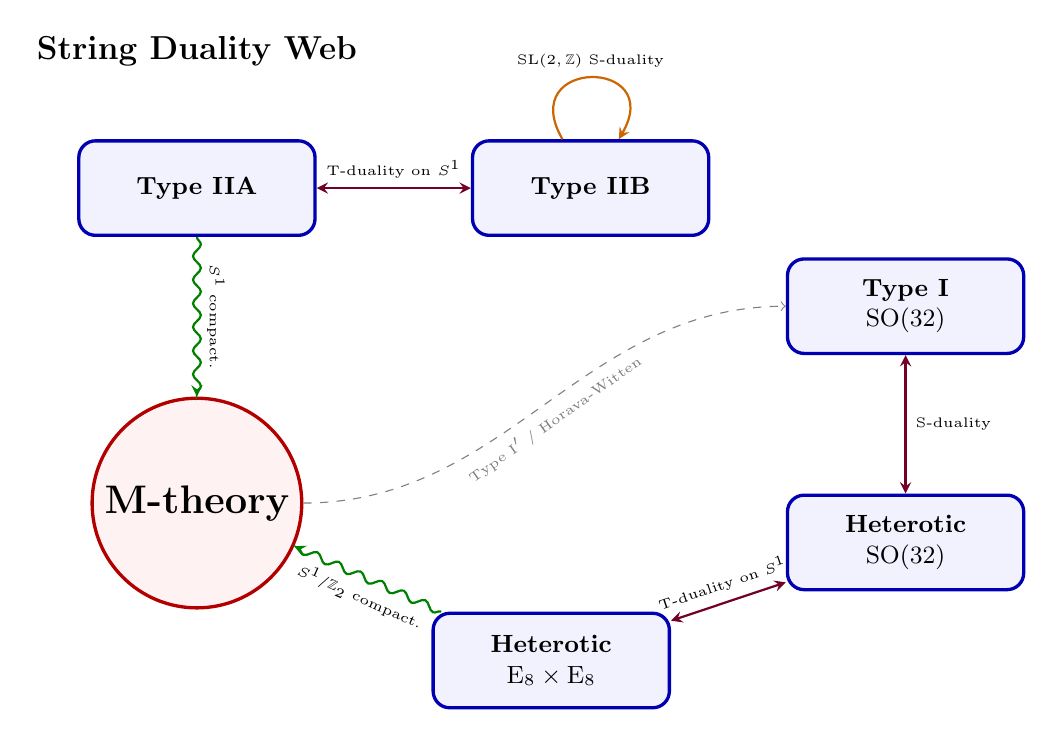
\begin{tikzpicture}[
    node distance = 3.5cm and 4.5cm,
    theory/.style = {rectangle, rounded corners=6pt, draw=blue!70!black, fill=blue!5, very thick, minimum width=3.0cm, minimum height=1.2cm, align=center, font=\small\bfseries},
    mtheory/.style = {circle, draw=red!70!black, fill=red!5, very thick, minimum size=2.4cm, align=center, font=\bfseries},
    duality/.style = {<->, >=stealth, thick, draw=purple!60!black},
    compact/.style = {->, >=stealth, thick, draw=green!50!black, decorate, decoration={snake, amplitude=0.5mm, segment length=3mm}},
    selfdual/.style = {->, >=stealth, thick, draw=orange!80!black, out=120, in=60, loop, distance=1.2cm}
]

% Node placement: a hexagon-like arrangement with M-theory at bottom center
\node[theory] (IIA) at (0,3) {Type IIA};
\node[theory] (IIB) at (5,3) {Type IIB};
\node[theory] (I) at (9,1.5) {Type I\\$\mathrm{SO}(32)$};
\node[theory] (HETSO) at (9,-1.5) {Heterotic\\$\mathrm{SO}(32)$};
\node[theory] (HETE8) at (4.5,-3) {Heterotic\\$\mathrm{E}_8\times\mathrm{E}_8$};
\node[mtheory] (M) at (0,-1) {\Large M-theory};

% T-duality between IIA and IIB
\draw[duality] (IIA) -- node[above, midway, font=\tiny] {T-duality on $S^1$} (IIB);

% T-duality between heterotic theories
\draw[duality] (HETSO) -- node[above, sloped, font=\tiny] {T-duality on $S^1$} (HETE8);

% S-duality between I and HETSO
\draw[duality] (I) -- node[right, midway, font=\tiny] {S-duality} (HETSO);

% IIB self S-duality
\draw[selfdual] (IIB) to node[above, font=\tiny] {$\mathrm{SL}(2,\mathbb{Z})$ S-duality} (IIB);

% Connections to M-theory
\draw[compact] (IIA) -- node[sloped, above, font=\tiny] {$S^1$ compact.} (M);
\draw[compact] (HETE8) -- node[sloped, below, font=\tiny] {$S^1/\mathbb{Z}_2$ compact.} (M);

% Additional connection from M-theory to I and HETSO via orientifold (optional dashed line)
\draw[dashed, gray, ->] (M) to[out=0, in=180] node[below, sloped, font=\tiny, gray] {Type I$'$ / Horava-Witten} (I);

% Title
\node[above=0.8cm of IIA, font=\large\bfseries] {String Duality Web};

\end{tikzpicture}
\caption{The web of string dualities. Arrows indicate equivalences between theories in the appropriate limits. T-duality links the two Type II theories and the two heterotic theories. S-duality connects Type I and Heterotic $\mathrm{SO}(32)$, while Type IIB is self-dual under $\mathrm{SL}(2,\mathbb{Z})$. The strong-coupling limits of Type IIA and Heterotic $\mathrm{E}_8\times\mathrm{E}_8$ are described by eleven-dimensional M-theory compactified on a circle or an interval, respectively. The dashed line indicates a more subtle connection via orientifolds and Horava--Witten theory. All five perturbative string theories and eleven-dimensional supergravity are thus unified in the moduli space of a single non-perturbative theory.}
\label{fig:dualityweb}
\end{figure}

The diagram illustrates that:
\begin{itemize}
    \item Type IIA and Type IIB are related by T-duality on a circle.
    \item The two heterotic theories are also related by T-duality on a circle.
    \item Type I and Heterotic $\mathrm{SO}(32)$ are S-dual.
    \item Type IIB is self-S-dual under $\mathrm{SL}(2,\mathbb{Z})$.
    \item M-theory on a circle gives Type IIA string theory.
    \item M-theory on an interval $S^1/\mathbb{Z}_2$ gives Heterotic $\mathrm{E}_8\times\mathrm{E}_8$.
    \item Furthermore, Type I$'$ (Type I with D9-branes and D5-branes) can be obtained from M-theory on $T^2/\mathbb{Z}_2$, completing the web.
\end{itemize}

Because all five theories are connected by dualities, they are no longer viewed as distinct. Instead, they represent different perturbative expansions around different points in the moduli space of a single underlying theory---M-theory.

\section{Implications and Concluding Remarks}
String dualities have revolutionized our understanding of string theory. Some key implications are:
\begin{itemize}
    \item \textbf{Uniqueness of M-theory}: The five ten-dimensional superstring theories and eleven-dimensional supergravity are unified into a single non-perturbative framework. At present, a complete formulation of M-theory is lacking, but its existence is strongly supported by the web of dualities.
    \item \textbf{Brane democracy}: D-branes, NS5-branes, M2- and M5-branes, and other extended objects are all on equal footing. Their tensions and charges are constrained by duality symmetries.
    \item \textbf{Moduli spaces and U-duality}: The moduli spaces of string compactifications are often given by coset spaces modulo discrete U-duality groups. This has profound consequences for string phenomenology and cosmology.
    \item \textbf{Non-perturbative effects}: S-duality, in particular, provides a window into non-perturbative phenomena such as instantons and monopoles, which are essential for addressing issues like supersymmetry breaking and moduli stabilization.
\end{itemize}

In conclusion, string dualities have transformed string theory from a collection of five independent perturbative theories into a single, albeit still mysterious, overarching structure. They lie at the heart of the modern understanding that string theory is not just a theory of strings but of a much richer spectrum of branes and geometries, ultimately hinting at the existence of M-theory.

\appendix
\section{Supergravity Actions and Duality Symmetries}

In this appendix, we provide a brief overview of the low-energy effective supergravity actions for the various string theories and highlight how duality symmetries are realized at the level of the classical field equations.

\subsection{Type IIB Supergravity and $\mathrm{SL}(2,\mathbb{R})$ Symmetry}

The bosonic sector of ten-dimensional Type IIB supergravity consists of the metric $g_{MN}$, the dilaton $\Phi$, the Kalb--Ramond 2-form $B_2$, the Ramond--Ramond $p$-form potentials $C_0$, $C_2$, and $C_4$ (with a self-dual field strength). The action in the string frame takes the form
\begin{equation}
\begin{aligned}
S_{\text{IIB}} = \frac{1}{2\kappa_{10}^2} \int d^{10}x \sqrt{-g} \Biggl\{
&e^{-2\Phi} \left( R + 4 (\partial \Phi)^2 - \frac{1}{12} |H_3|^2 \right) \\
&- \frac{1}{2} |F_1|^2 - \frac{1}{12} |\widetilde{F}_3|^2 - \frac{1}{480} |\widetilde{F}_5|^2 \Biggr\} \\
&+ \frac{1}{4\kappa_{10}^2} \int C_4 \wedge H_3 \wedge F_3 + \text{fermions},
\end{aligned}
\end{equation}
where
\begin{align}
H_3 &= d B_2, \\
F_p &= d C_{p-1}, \quad p=1,3,5, \\
\widetilde{F}_3 &= F_3 - C_0 \wedge H_3, \\
\widetilde{F}_5 &= F_5 - \frac{1}{2} C_2 \wedge H_3 + \frac{1}{2} B_2 \wedge F_3,
\end{align}
and the self-duality constraint $\widetilde{F}_5 = \star \widetilde{F}_5$ must be imposed by hand at the level of the equations of motion.

Introduce the axio-dilaton
\begin{equation}
\tau = C_0 + i e^{-\Phi}.
\end{equation}
The action is manifestly invariant under the $\mathrm{SL}(2,\mathbb{R})$ transformation
\begin{equation}
\tau \to \frac{a\tau + b}{c\tau + d}, \qquad 
\begin{pmatrix} a & b \\ c & d \end{pmatrix} \in \mathrm{SL}(2,\mathbb{R}),
\end{equation}
provided the 2-forms transform as a doublet
\begin{equation}
\begin{pmatrix} B_2 \\ C_2 \end{pmatrix} \to 
\begin{pmatrix} a & b \\ c & d \end{pmatrix} \begin{pmatrix} B_2 \\ C_2 \end{pmatrix},
\end{equation}
while $C_4$ and the Einstein-frame metric are invariant. The Einstein-frame metric is related to the string-frame metric by $g_{MN}^{\text{E}} = e^{-\Phi/2} g_{MN}^{\text{S}}$.

At the quantum level, the continuous $\mathrm{SL}(2,\mathbb{R})$ symmetry is broken to the discrete subgroup $\mathrm{SL}(2,\mathbb{Z})$ by the presence of D$(-1)$-brane instantons (which couple to $C_0$) and by the Dirac quantization conditions for the charges of D-strings and fundamental strings. This $\mathrm{SL}(2,\mathbb{Z})$ is an exact non-perturbative symmetry of Type IIB string theory.

\subsection{Eleven-Dimensional Supergravity}

The low-energy limit of M-theory is described by eleven-dimensional supergravity. The bosonic action contains only the metric $G_{MN}$ and a 3-form potential $A_3$ with field strength $F_4 = dA_3$:
\begin{equation}
S_{11} = \frac{1}{2\kappa_{11}^2} \int d^{11}x \sqrt{-G} \left( R - \frac{1}{48} |F_4|^2 \right) 
- \frac{1}{12\kappa_{11}^2} \int A_3 \wedge F_4 \wedge F_4 + \text{fermions}.
\end{equation}
This action is unique and has no continuous free parameters (other than the eleven-dimensional Planck length $\ell_{11}$, which sets the scale). The absence of a dilaton is a hallmark of M-theory; the string coupling emerges only upon compactification.

Dimensional reduction of $S_{11}$ on a circle $S^1$ yields the Type IIA supergravity action. Explicitly, using the ansatz
\begin{equation}
ds_{11}^2 = e^{-2\Phi/3} ds_{10}^2 + e^{4\Phi/3} (dx^{11} + C_1)^2,
\end{equation}
and identifying components of $A_3$ with the NS-NS 2-form $B_2$ and the RR 3-form $C_3$ of Type IIA, one recovers the IIA action with its characteristic dilaton coupling. The radius of the eleventh dimension is
\begin{equation}
R_{11} = g_s^{2/3} \ell_s,
\end{equation}
where $g_s = e^{\langle \Phi \rangle}$ is the Type IIA string coupling and $\ell_s = \sqrt{\alpha'}$ is the string length. This geometric relation is the essence of the S-duality connection between Type IIA and M-theory.

\subsection{T-Duality in Supergravity}

T-duality can also be understood directly at the level of the low-energy supergravity actions. Consider the reduction of the common NS-NS sector (metric, dilaton, and $B$-field) on a circle of radius $R$. The dimensionally reduced action in $D=9$ possesses an $\mathrm{O}(1,1;\mathbb{R})$ symmetry (scaling symmetry) that is promoted to $\mathrm{O}(1,1;\mathbb{Z})$ in the full string theory. This is the T-duality group for a single circle.

For toroidal compactifications on $T^d$, the moduli space of the NS-NS sector is the coset
\begin{equation}
\mathcal{M}_{d,d} = \mathrm{O}(d,d;\mathbb{R}) / \bigl( \mathrm{O}(d;\mathbb{R}) \times \mathrm{O}(d;\mathbb{R}) \bigr),
\end{equation}
and the discrete T-duality group is $\mathrm{O}(d,d;\mathbb{Z})$. The action of T-duality mixes the metric $G_{ij}$ and the internal $B$-field $B_{ij}$ in a non-trivial way. For $d=1$, the transformation reduces to the familiar Buscher rules:
\begin{align}
G'_{99} &= \frac{1}{G_{99}}, \qquad e^{2\Phi'} = \frac{e^{2\Phi}}{G_{99}}, \\
B'_{\mu 9} &= B_{\mu 9} + \frac{G_{\mu 9}}{G_{99}}, \qquad G'_{\mu 9} = \frac{B_{\mu 9}}{G_{99}}, \quad \text{etc.}
\end{align}
where $\mu$ runs over the non-compact directions and $9$ denotes the compact circle.

\subsection{U-Duality and Exceptional Groups}

When the RR fields are included, the moduli space of Type II theories on $T^d$ enlarges. The full U-duality group can be derived by considering M-theory on $T^{d+1}$ and then reducing to ten dimensions. The continuous symmetries of the supergravity action form a non-compact exceptional group $E_{d+1(d+1)}(\mathbb{R})$, and the discrete U-duality group is its integer form $E_{d+1(d+1)}(\mathbb{Z})$.

For instance, in the maximal case of M-theory on $T^8$, the moduli space is
\begin{equation}
\mathcal{M} = E_{8(8)}(\mathbb{Z}) \backslash E_{8(8)}(\mathbb{R}) / \bigl( \mathrm{Spin}(16) / \mathbb{Z}_2 \bigr),
\end{equation}
where the denominator is the maximal compact subgroup of $E_{8(8)}$. The U-duality group contains both the T-duality $\mathrm{O}(7,7;\mathbb{Z})$ of the Type II string on $T^7$ and the S-duality $\mathrm{SL}(2,\mathbb{Z})$ of the Type IIB theory in a unified fashion.

The existence of these exceptional symmetries in the low-energy effective action is a powerful constraint on quantum corrections. For instance, in $N=8$ supergravity in four dimensions (arising from M-theory on $T^7$), the continuous $E_{7(7)}(\mathbb{R})$ symmetry is believed to be broken to the discrete $E_{7(7)}(\mathbb{Z})$ by quantum effects, which is exactly the U-duality group of the full string/M-theory. This has been used to argue for the finiteness of certain $N=8$ supergravity amplitudes.

In summary, the supergravity actions exhibit continuous global symmetries that are the classical precursors to the exact discrete dualities of the full quantum string/M-theory. The duality web is deeply imprinted in the structure of the low-energy effective field theories.

\begin{thebibliography}{9}
\bibitem{witten95} E. Witten, ``String theory dynamics in various dimensions,'' Nucl.\ Phys.\ B \textbf{443}, 85 (1995) [hep-th/9503124].
\bibitem{hull94} C. M. Hull and P. K. Townsend, ``Unity of superstring dualities,'' Nucl.\ Phys.\ B \textbf{438}, 109 (1995) [hep-th/9410167].
\bibitem{polchinski} J. Polchinski, \textit{String Theory}, Cambridge University Press, 1998.
\bibitem{becker} K. Becker, M. Becker and J. H. Schwarz, \textit{String Theory and M-Theory: A Modern Introduction}, Cambridge University Press, 2006.
\end{thebibliography}

\end{document}